\documentclass[../../main.tex]{subfiles}

\graphicspath{{../../fig/}}
\setcounter{section}{0}

\begin{document}

\chapter{宇宙マイクロ波背景放射(CMB)偏光観測}
宇宙マイクロ波背景放射(Cosmic Microwave Background: CMB)とは、宇宙の創生から38万年後に物質から脱結合した光子のことであり、我々が観測できる最古の光である。
その発見はペンジアスとウィルソンによって1965年に行われ\cite{1965ApJ...142..419P}、
その後Cosmic Background Explorer(COBE)衛星により強度の周波数依存性(スペクトル)が測定された\cite{1996ApJ...473..576F}。
測定されたスペクトルは温度が$\SI{2.725}{K}$の黒体輻射のスペクトルと一致し(図\ref{fig:cobe})、
CMBの強度が天球面上の各点においてわずかな違いはあれど、ほとんど一様等方であることも確認された。
この事実はかつて宇宙が熱平衡状態にあったことを示し、宇宙が高温高密度の状態から膨張して現在に至るビッグバン宇宙モデルを支持する強力な証拠となった。
こうして現代の宇宙論の基礎を築き、発展させてきたCMBは、現在ではその偏光情報からインフレーション宇宙論の証拠を探ることができると期待されている。

本章では、はじめに現在の標準的な宇宙モデルである$\Lambda\mathrm{CDM}$モデルの概要と抱える問題について述べ、
次いでその問題の解決策としてインフレーション宇宙論について述べる。
その後、インフレーションがCMBパワースペクトルにどのような変化をもたらすかについて述べ、最後に本論文の構成について述べる。

\colortext{red}{最後の本章で〜の部分は最後に考える。}
\begin{figure}[H]
    \centering
    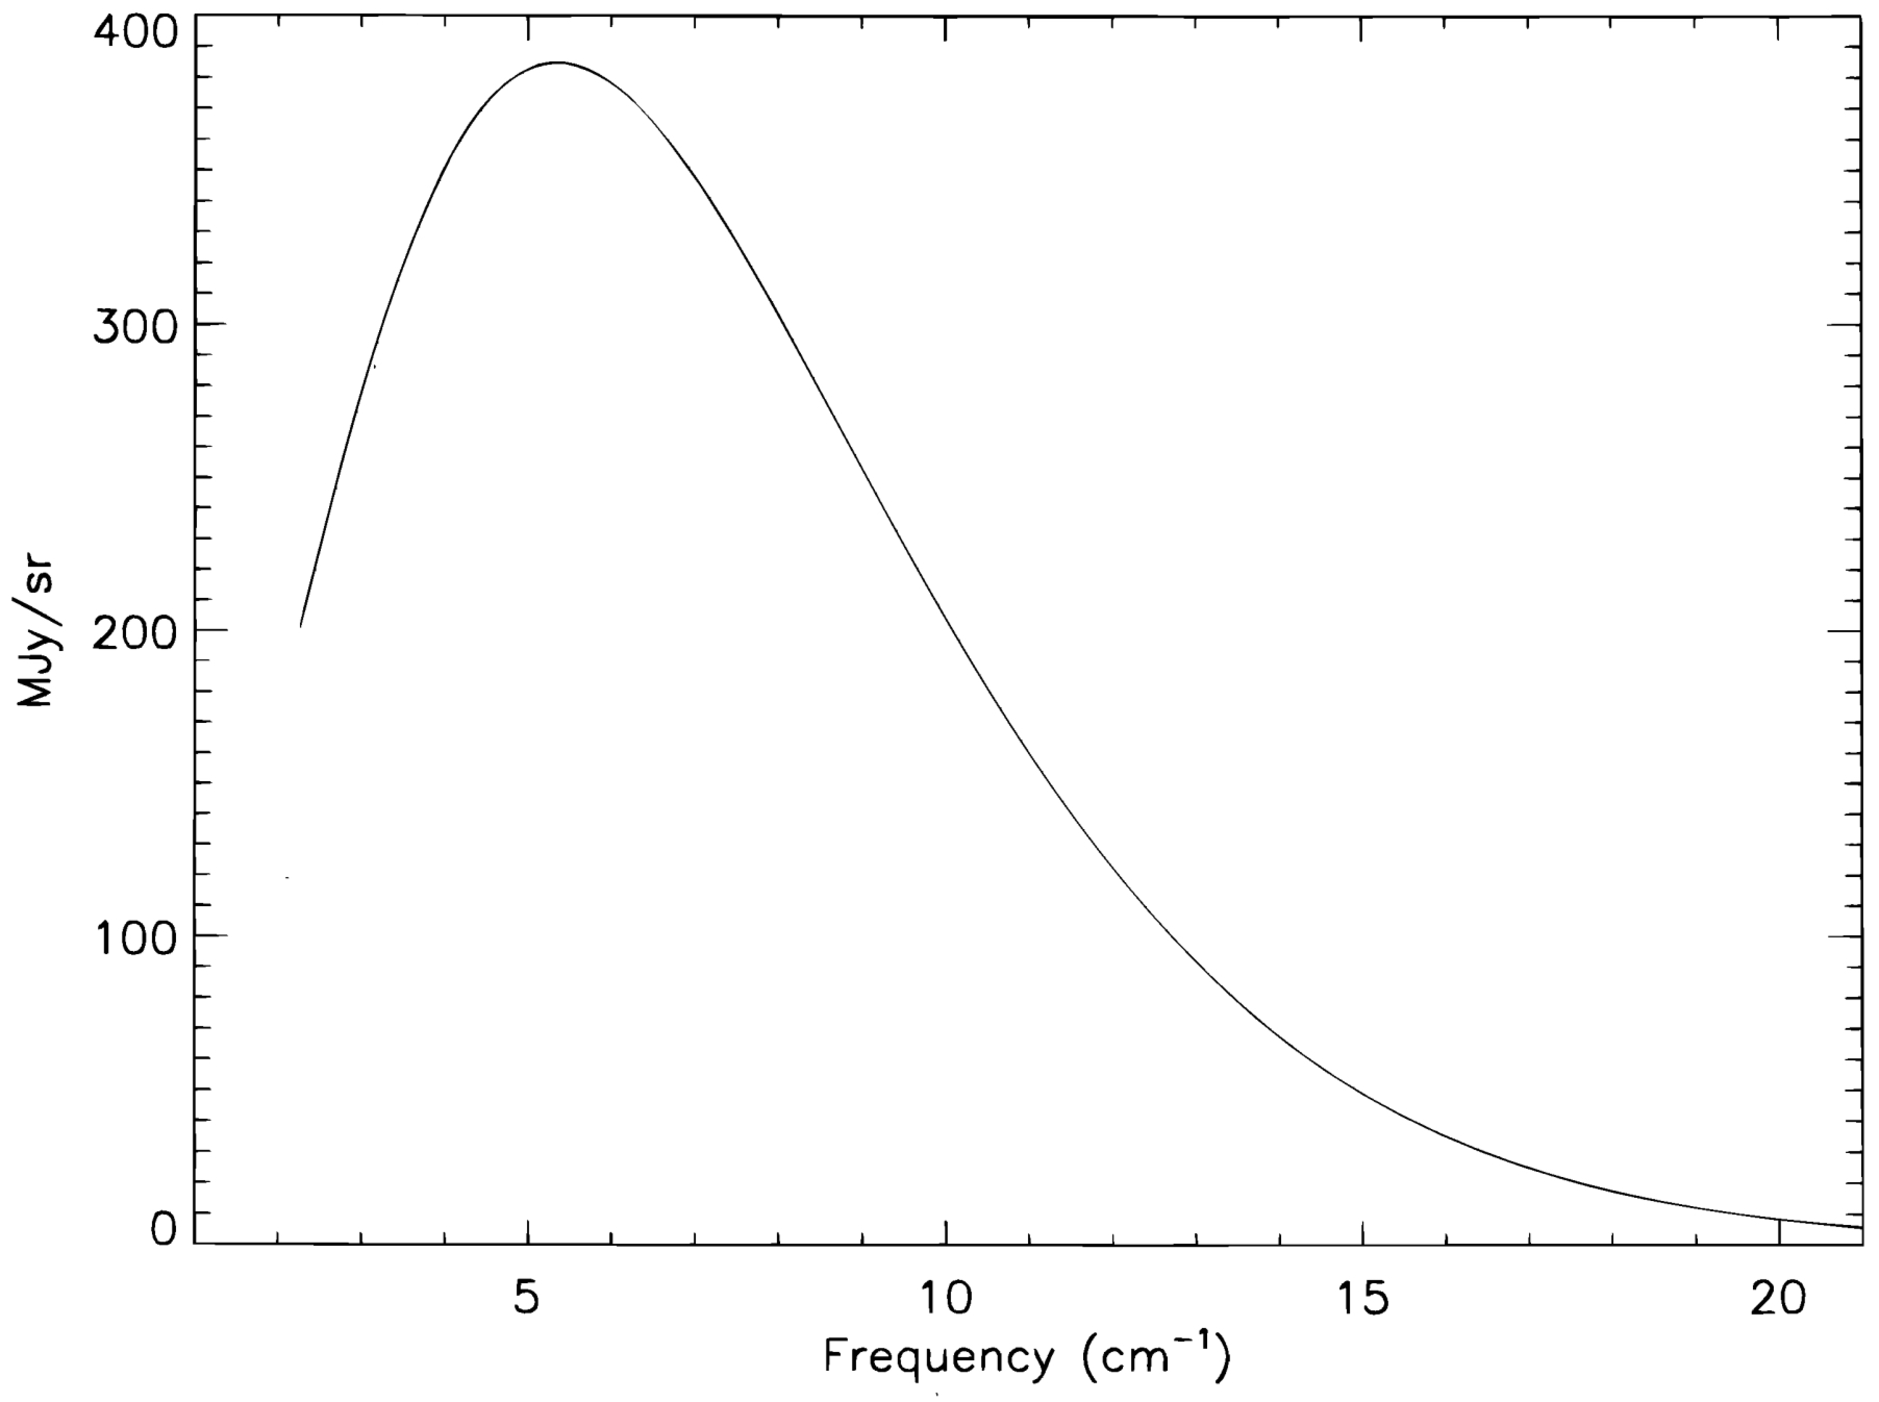
\includegraphics[width=0.6\textwidth]{intro/cobe.pdf}
    \caption{COBE衛星によるCMBのスペクトル測定値を黒体輻射のスペクトルでfittingした結果。}
    \label{fig:cobe}
\end{figure}

\section{$\Lambda\mathrm{CDM}$モデル}
現在の標準的な宇宙モデルである$\Lambda\mathrm{CDM}$モデルについて述べる。
まず、Einstein方程式は、計量テンソル$g_{\mu\nu}$、Einsteinテンソル$G_{\mu\nu}$とエネルギー運動量テンソル$T_{\mu\nu}$を用いて
\begin{equation}
    \label{eq:einstein}
    G_{\mu\nu}+\Lambda g_{\mu\nu}=8\pi GT_{\mu\nu}
\end{equation}
とかける。ここで、$G$は重力定数、$\Lambda$は宇宙定数である。また、自然単位系を採用した。
一様等方な宇宙では、その計量はフリードマン・ルメートル・ロバートソン・ウォーカー計量
\begin{equation}
    \label{eq:rwmetric}
    ds^2=-dt^2+a^2(t)\qty[\frac{dr^2}{1-Kr^2}+r^2d\Omega^2]
\end{equation}
で記述される。ここで、$a(t)$はスケールファクター、$K$は宇宙の曲率を表す。
また、宇宙の物質が完全流体であることを仮定すると、エネルギー運動量テンソルを
\begin{equation}
    \label{eq:emtensor}
    T_{\mu\nu}=\mqty(-\rho&0&0&0\\0&P&0&0\\0&0&P&0\\0&0&0&P)
\end{equation}
と表すことができる。ここで、$\rho$はエネルギー密度、$P$は圧力である。
エネルギー運動量テンソルを用いてエネルギー保存則を考えると
\begin{equation}
    \label{eq:energyconservation}
    \dot{\rho}+3\dfrac{\dot{a}}{a}(\rho+P)=0
\end{equation}
を得る。
式\eqref{eq:rwmetric}、式\eqref{eq:emtensor}を式\eqref{eq:einstein}に代入し、$(0,\,0)$に注目すると
\begin{align}
    \label{eq:friedmann}
    H^2:=\qty(\dfrac{\dot{a}}{a})^2 &= \dfrac{8\pi G}{3}\rho+\dfrac{\Lambda}{3}-\dfrac{K}{a^2}
\end{align}
を得る。これをフリードマン方程式と呼ぶ。$H:=\dot{a}/a$はハッブル定数である。
エネルギー密度$\rho$は、物質による寄与と放射による寄与とに大別することができる。
各々のエネルギー密度$\rho_m$、$\rho_r$はそれぞれ$a^{-3}$、$a^{-4}$に比例するため、フリードマン方程式は
\begin{equation}
    \label{eq:friedmann2}
    H^2=H_0^2\qty[\dfrac{\Omega_m}{a^3}+\dfrac{\Omega_r}{a^4}+\dfrac{\Omega_{K}}{a^2}+\Omega_{\Lambda}]
\end{equation}
と書ける。
ここで、$H_0$は現在のハッブル定数、$\Omega_m,\,\Omega_r,\,\Omega_{K},\,\Omega_{\Lambda}$はそれぞれ物質、放射、曲率、宇宙定数の密度パラメータであり
% 現在の各成分のエネルギー密度$\rho_{m,\,0},\,\rho_{r,\,0}$を用いて
\begin{align}
    \label{eq:omega}
    \Omega_m&:=\dfrac{8\pi G\rho_{m}}{3H_0^2},\quad
    \Omega_r:=\dfrac{8\pi G\rho_{r}}{3H_0^2},\quad
    \Omega_{K}:=\dfrac{-K}{H_0^2a^2},\quad
    \Omega_{\Lambda}:=\dfrac{\Lambda}{3H_0^2}
\end{align}
と表される。これらの密度パラメータは
\begin{equation}
    \label{eq:omegaconstraint}
    \Omega_{m}+\Omega_{r}+\Omega_{\Lambda}+\Omega_{K}=1
\end{equation}
を満たすが、これまでのCMBの観測は$\Omega_{m}+\Omega_{r}+\Omega_{\Lambda}=1$という結果を示しているため、宇宙は平坦であると考えられている\cite{Bennett_2003}。


$\Lambda\mathrm{CDM}$モデルには、以下の3つの問題をもつ。
\begin{enumerate}
    \item 地平線問題:CMBの温度揺らぎは天球面上のどの方向を見ても$\Delta T/T\sim 10^{-5}$と非常に小さい。
    これは因果関係を持たないはずの2点の温度が高い精度で一致していることを意味しており、$\Lambda\mathrm{CDM}$モデルはこの理由を説明できない。
    \item 平坦性問題:これまでの観測によれば、現在の宇宙は曲率がほとんどゼロである。宇宙の曲率の密度パラメータ$\Omega_{K}$は、時間発展とともに成長するため、
    宇宙初期に遡ると$\Omega_{K}$は不自然なほどに小さくなければならない。
    \item モノポール問題:大統一理論などの素粒子標準理論を超えた理論は、しばしば宇宙初期に磁気モノポールが生成されることを予言する。
    しかし、現在にいたるまで磁気モノポールは発見されていない。
\end{enumerate}
\section{インフレーションモデル}
前節にて述べた3つの問題の解決策として有力視されている理論が、
宇宙初期において宇宙が指数関数的に膨張したとするインフレーションモデルである。
この急激な膨張は因果律を持つ領域を急激に拡大し、空間を平坦にし、モノポールの濃度を薄めることで
地平線問題、平坦性問題、モノポール問題を解決することができる。

インフレーションモデルは佐藤、グースらによって1981年に提唱された\cite{10.1093/mnras/195.3.467}\cite{PhysRevD.23.347}が、
現在では多種多様なバリエーションを有する\cite{Tsujikawa_book}。
ここでは、宇宙初期にインフラトンというスカラー場$\phi$によって引き起こされ、
スローロール近似を課したインフレーションについて紹介する。

一様等方な宇宙のもとでのインフラトンの運動方程式は
\begin{equation}
    \ddot{\phi}+3H\dot{\phi}+c^2\pdv{V}{\phi} = 0
\end{equation}
と与えられる。$H$はハッブル定数である。
また、曲率$K=0$のフリードマン方程式\eqref{eq:friedmann}はインフラトンのエネルギー密度の寄与が主要であるとすると
\begin{equation}
    3H^2M_{\mathrm{pl}}^2 = \dfrac{1}{2c^2}\dot{\phi}^2 +V(\phi)
\end{equation}
となる。$M_{\mathrm{pl}}=\sqrt{1/8\pi G}$は換算プランク質量である。
ここで、スローロール近似と呼ばれる、インフレーションが十分長い時間続くための近似
\begin{align}
    \qty|\dfrac{\dot{\phi}^2}{V(\phi)}| \ll 1,\qquad \qty|\dfrac{\ddot{\phi}}{H\dot{\phi}}| \ll 1
\end{align}
を課す。式\eqref{}と\eqref{}から
\begin{align}
    H^2 &= \dfrac{V(\phi)}{3M_{\mathrm{pl}}} \\
    \dot{H} &= -\dfrac{\dot{\phi}}{2c^2M_{\mathrm{pl}}^2}
\end{align}
を得る。以上から、インフレーション中のスケール因子$a$は
\begin{align}
    a&\propto e^{\mathcal{N}} \\
    \mathcal{N} &:= -\int_{t_f}^{t}H\dd{\tilde{t}} = -\dfrac{1}{M_{\mathrm{pl}}^2}\int_{\phi_f}^{\phi}\dfrac{V}{\partial V/\partial \phi}\dd{\tilde{\phi}}
\end{align}
のように指数関数的に増えていく。ここで、$t$はインフレーション中の時刻、$t_f$はインフレーションが終わる時刻であり、
$\phi_f$はインフレーションが終わる時刻での$\phi$である。

インフレーションにおけるスケール因子の指数関数的増加は空間の指数関数的膨張を引き起こす。
時空が量子化されていると仮定し、
\section{CMB偏光モード}
\section{本論文の構成}

\end{document}